\documentclass[10.5pt]{article}
\usepackage[T1]{fontenc}
\usepackage{graphicx}
\usepackage{hyperref}
\usepackage[small]{titlesec}

\setlength{\oddsidemargin}{0in}
\setlength{\textwidth}{6.5in}
\setlength{\topmargin}{0in}
\setlength{\textheight}{8.5in}

\begin{document}

\title{\textbf{Detecting Type of Tennis Shots from Broadcast Video}}
\author{Kunal Vyas\\
    University of Massachusetts Lowell\\
  \texttt{kunal\_vyas@student.uml.edu}
  \and
  Eugene Stanley\\
  University of Massachusetts Lowell\\
  \texttt{eugene\_stanley@student.uml.edu}}
  \date{\vspace{-1ex}}
  \maketitle
  
  \section{Team members and roles:}
  We are going to work on this project in a team of \textit{two}:\\
  \\
    \textit{ - Kunal} (Graduate student) : Problem Analysis, Algorithm Development, Research, Code implementation, Dataset Analysis, Interface development, Testing, Debugging\\
    \textit{ - Eugene} (Undergraduate student) : Research, Code implementation, Documentation, Algorithm Development, Testing and Debugging.
    \section{Goal:}
    Watching professional tennis players play is the most important and fundamental way to improve one's own game. By observing certain statistics like the kind of shots hit during a tennis match, people can learn from what the professionals do and improve their own game.\\
    \\
    Shots could be classified by type so that they can be indexed and retrieved later for studying a particular shot technique. Video archives or old tennis matches could be \underline{data mined} to provide a novice examples of the requested shot. Our goal is to create an application which can accurately and quickly categorize shots by various type.
    \begin{figure}[h]
    \centering
    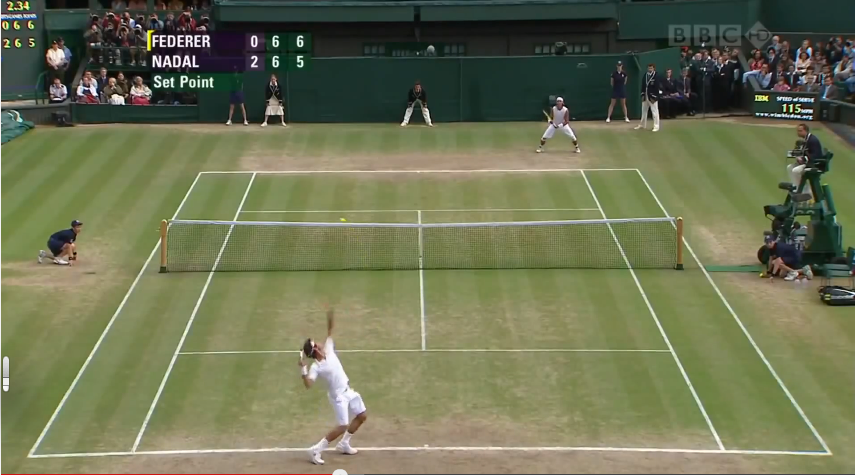
\includegraphics[width=0.32\textwidth]{serve.png}
    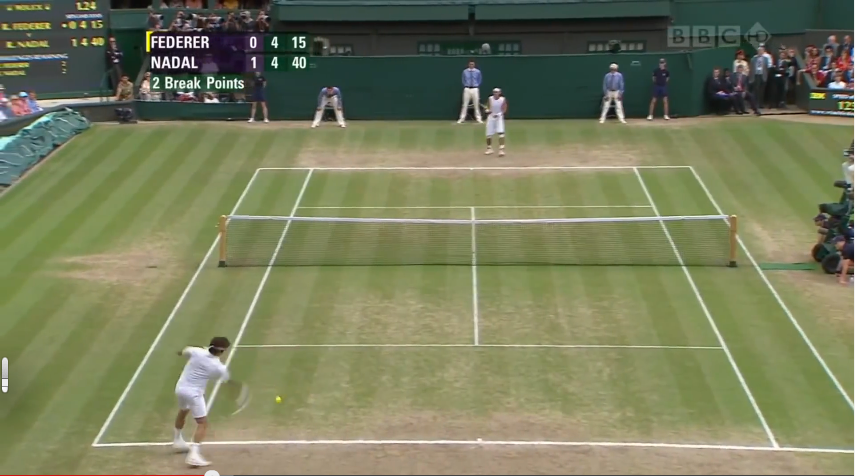
\includegraphics[width=0.32\textwidth]{forehand.png}
    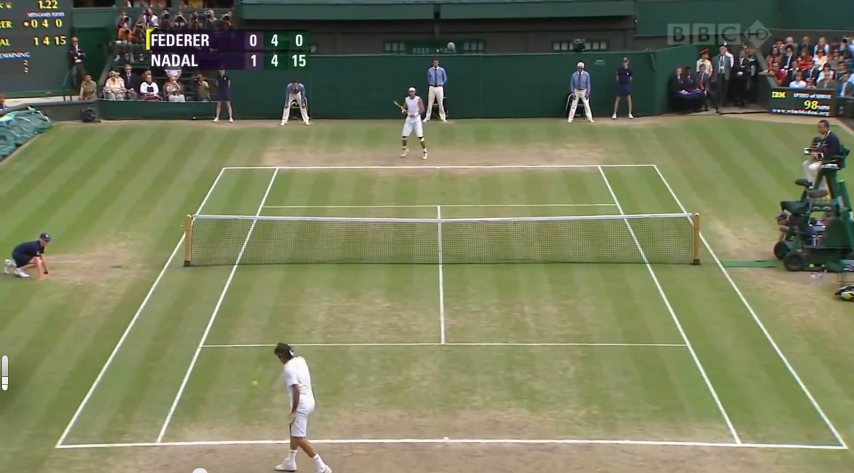
\includegraphics[width=0.32\textwidth]{backhand.png}
    \caption{The three basic shots that a player hits in Tennis: \textit{Serve}, \textit{Forehand} and the \textit{Backhand}}
    \end{figure}
    
    \section{Motivation:}
    The motivation for this project comes from the need of match statistics which are often displayed after the matches. We think it is important to gather as many facts as possible because they can help in analysis and allow for degrees of improvement by learning from mistakes.
    
    \section{Existing Work:}
    There are existing implementations that serve the same purpose:
    \subsection{CS229: Action Recognition in Tennis\cite{stanford2012}}
        This method was developed by Aman Sikka and Rajbir Kataria at Stanford University in 2012. It learns the three Tennis actions by using Support Vector Machines (SVMs) classifier. Accuracy is inconsistent and so we plan to get better results from our method.
    \subsection{Player Action Recognition in Broadcast Tennis Video with Applications to Semantic Analysis of Sports Game\cite{asians}}
    This method was developed by Guangyu Zhu, Changsheng Xu, Qingming Huang, Wen Gao and Liyuan Xing in 2006. It considers the mapping relationship between relative movements of different body parts and the regions in the image plane.
    \subsection{Action Recognition in Tennis Videos using Optical Flow and Conditional Random Fields\cite{argentina}}
    This proposed approach combines the application of video processing techniques for region of interest detection and feature extraction in tennis videos, and CRFs for action recognition.\\
    \\
\textbf{Conclusion:} Although these and many more such implementations exist that are detecting activity of players, they are not accurate enough and we aim to improve that in our approach.
    \section{Approach:}
    Our approach will be to first detect the position of the ball and the players. We will detect the player using OpenCV's \textit{HOG descriptor}\cite{hog} for people detection. And we will detect the ball using \textit{Tennis Ball Tracking Algorithm for Automatic Annotation of Tennis Match}\cite{surrey}. Through this, we will decide if the shot has been hit. After detecting a successful hit, our program will analyze the frames around which the hit occurred to determine whether the type of shot used was a forehand, smash, or backhand shot. It is a backhand if the ball is hit from the right and a forehand if it is from the left\footnote{We will have a flag for changing this for left handed players}.
    
    \section{Expected:}
    The application will take broadcast video as input and output the type of shot being performed for each successful hit. For a miss, it will report the type of shot used by the opposing player which caused it. It will also track each point and keep a score of the entire match.
    
    \section{Evaluation:}
    We will use \textit{C++} using the \textit{OpenCV} framework to develop this project. We are planning to use the \textit{ACASVA Actions Dataset}\cite{acasva} to determine if a player has hit a shot or not. The dataset when fed with input, determines one of three values -- serve, hit or non-hit. After evaluating this, we know if the ball has been hit by the player or not. To know the position of the player, we are going to use OpenCV's \texttt{gpu::HOGDescriptor}\cite{hog} class. Then we can determine the stroke type from the position of the player and the ball.

\begin{thebibliography}{99}

\bibitem{hog}
OpenCV Object Detection. \\
\href{http://docs.opencv.org/modules/gpu/doc/object\_detection.html}{\texttt{http://docs.opencv.org/modules/gpu/doc/object\_detection.html}}

\bibitem{surrey}
Yan, F, Christmas, W and Kittler, J (2005) A Tennis Ball Tracking Algorithm for Automatic Annotation of Tennis Match In: British Machine Vision Conference, 2005-09-05 - 2005-09-08, Oxford, UK.

\bibitem{stanford2012}
Aman Sikka, Rajbir Kataria (2012) CS229: Action Recognition in Tennis, Stanford University, Stanford, CA -- 94305.\\
\href{http://cs229.stanford.edu/proj2012/KatariaSikka-ActionRecognitionInTennis.pdf}{\texttt{http://cs229.stanford.edu/proj2012/KatariaSikka-ActionRecognitionInTennis.pdf}}

\bibitem{asians}
Guangyu Zhu, Changsheng Xu, Qingming Huang, Wen Gao and Liyuan Xing (2006). Player Action Recognition in Broadcast Tennis Video with Applications to Semantic Analysis of Sports Game. 

\bibitem{argentina}
Jo\'se F. Manera, Jonathan Vainstein,Claudio Delrieux and Ana Maguitman (2013). Action Recognition in Tennis Videos using Optical Flow and Conditional Random Fields.
\href{http://42jaiio.sadio.org.ar/proceedings/simposios/Trabajos/AST/14.pdf}{\texttt{http://42jaiio.sadio.org.ar/proceedings/simposios/Trabajos/AST/14.pdf}}

\bibitem{acasva}
Adaptive Cognition  for Automated Sports Video Annotation.\\
\href{http://www.cvssp.org/acasva/Downloads}{\texttt{http://www.cvssp.org/acasva/Downloads}}

\bibitem{}
\href{http://en.wikipedia.org/wiki/Activity\_recognition}{\texttt{http://en.wikipedia.org/wiki/Activity\_recognition}}

\bibitem{}
Terence Bloom and Andrew P. Bradley. Player Tracking and Stroke Recognition in Tennis Video
\href{{http://espace.library.uq.edu.au/eserv.php?pid=UQ:8928\&dsID=WDIC03\_Bloom.pdf}}{\texttt{http://espace.library.uq.edu.au/eserv.php?pid=UQ:8928\&dsID=WDIC03\_Bloom.pdf}}

\end{thebibliography}

\end{document} 